\subsubsection{Modellentwicklung am Objekt}
Nachdem das Testmodell (vgl. Abbildung \ref{fig:print-case-test_04}) nicht zu 100 \% gepasst hat, hat Manuel Starz die Abmessungen neu geklärt und diese in Fusion 360 übertragen (vgl. \ref{case_footprint}). Um Material für den 3D-Druck zu sparen, wurde die Zeichnung dann im Maßstab 1:1 auf Papier gedruckt, ausgeschnitten und angelegt.\par
Da hier einige Maße noch nicht gestimmt haben, hat Manuel Starz den Plan überarbeitet (vgl. \ref{case_footprint_final}). Diese neuen Bemaßungen waren dann korrekt.\par
Daraufhin wurde dann die Zeichnung in zwei eigenständige Dateien gesplittet, um die linke und die rechte Seite des Gehäuses zu konstruieren.\par
Die Grundabmessung des Bildschirms werden in Fusion 360 als neue Zeichnung angelegt. Hierzu wurde ein einfaches Rechteck mit den entsprechenden Außenmaßen angelegt (vlg. \ref{fig:design-case-01}). Anschließend wurden die Ecken mit einem Radius von 7mm abgerundet. (vgl. \ref{fig:design-case-02}). Abschließend wurde die Zeichnung in der Mitte geteilt, um die beiden Hälften des Gehäuses unabhängig\par
\begin{figure}[h!tb]
	\begin{subfigure}[b]{.5\linewidth}
		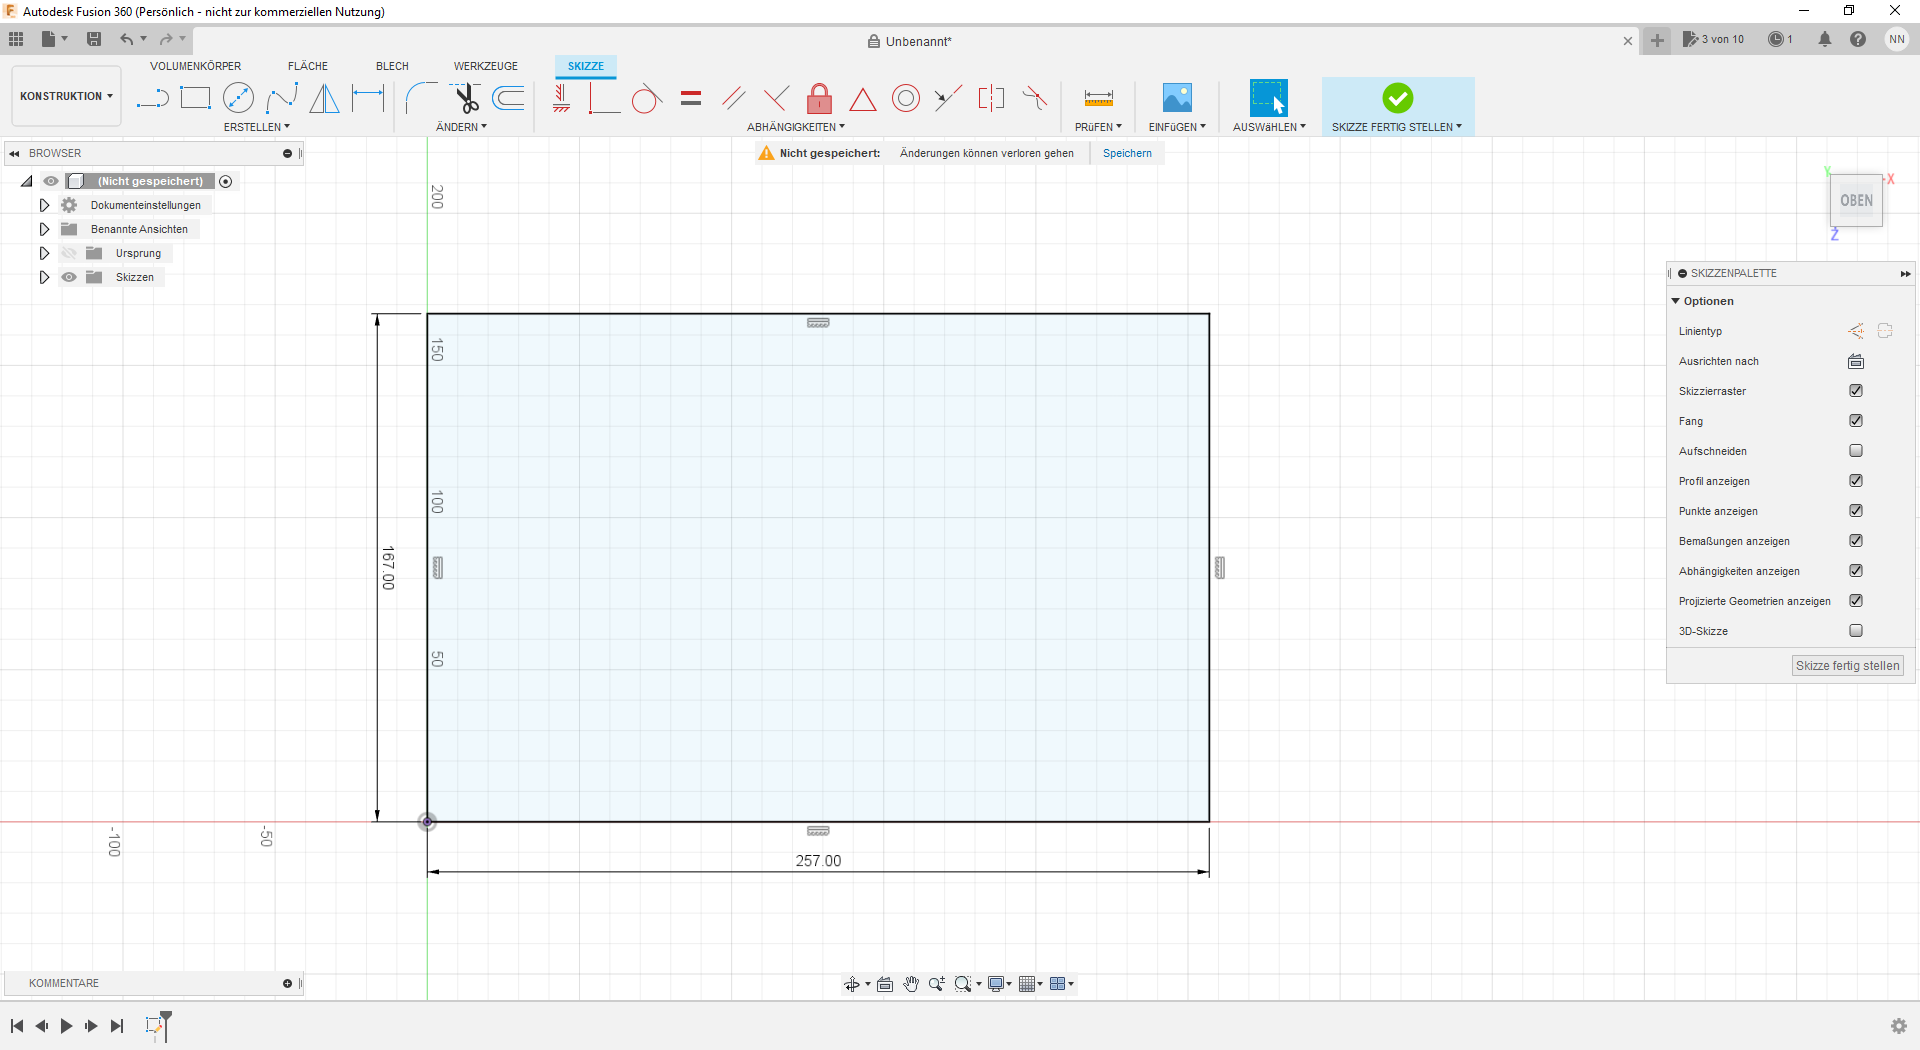
\includegraphics[width=1\textwidth]{img/konstruktion_gehaeuse_001.png}
		\caption[Zeichnen der Außenmaße]{Zeichnen der Außenmaße}
		\label{fig:design-case-01}
	\end{subfigure}
	\begin{subfigure}[b]{.5\linewidth}
		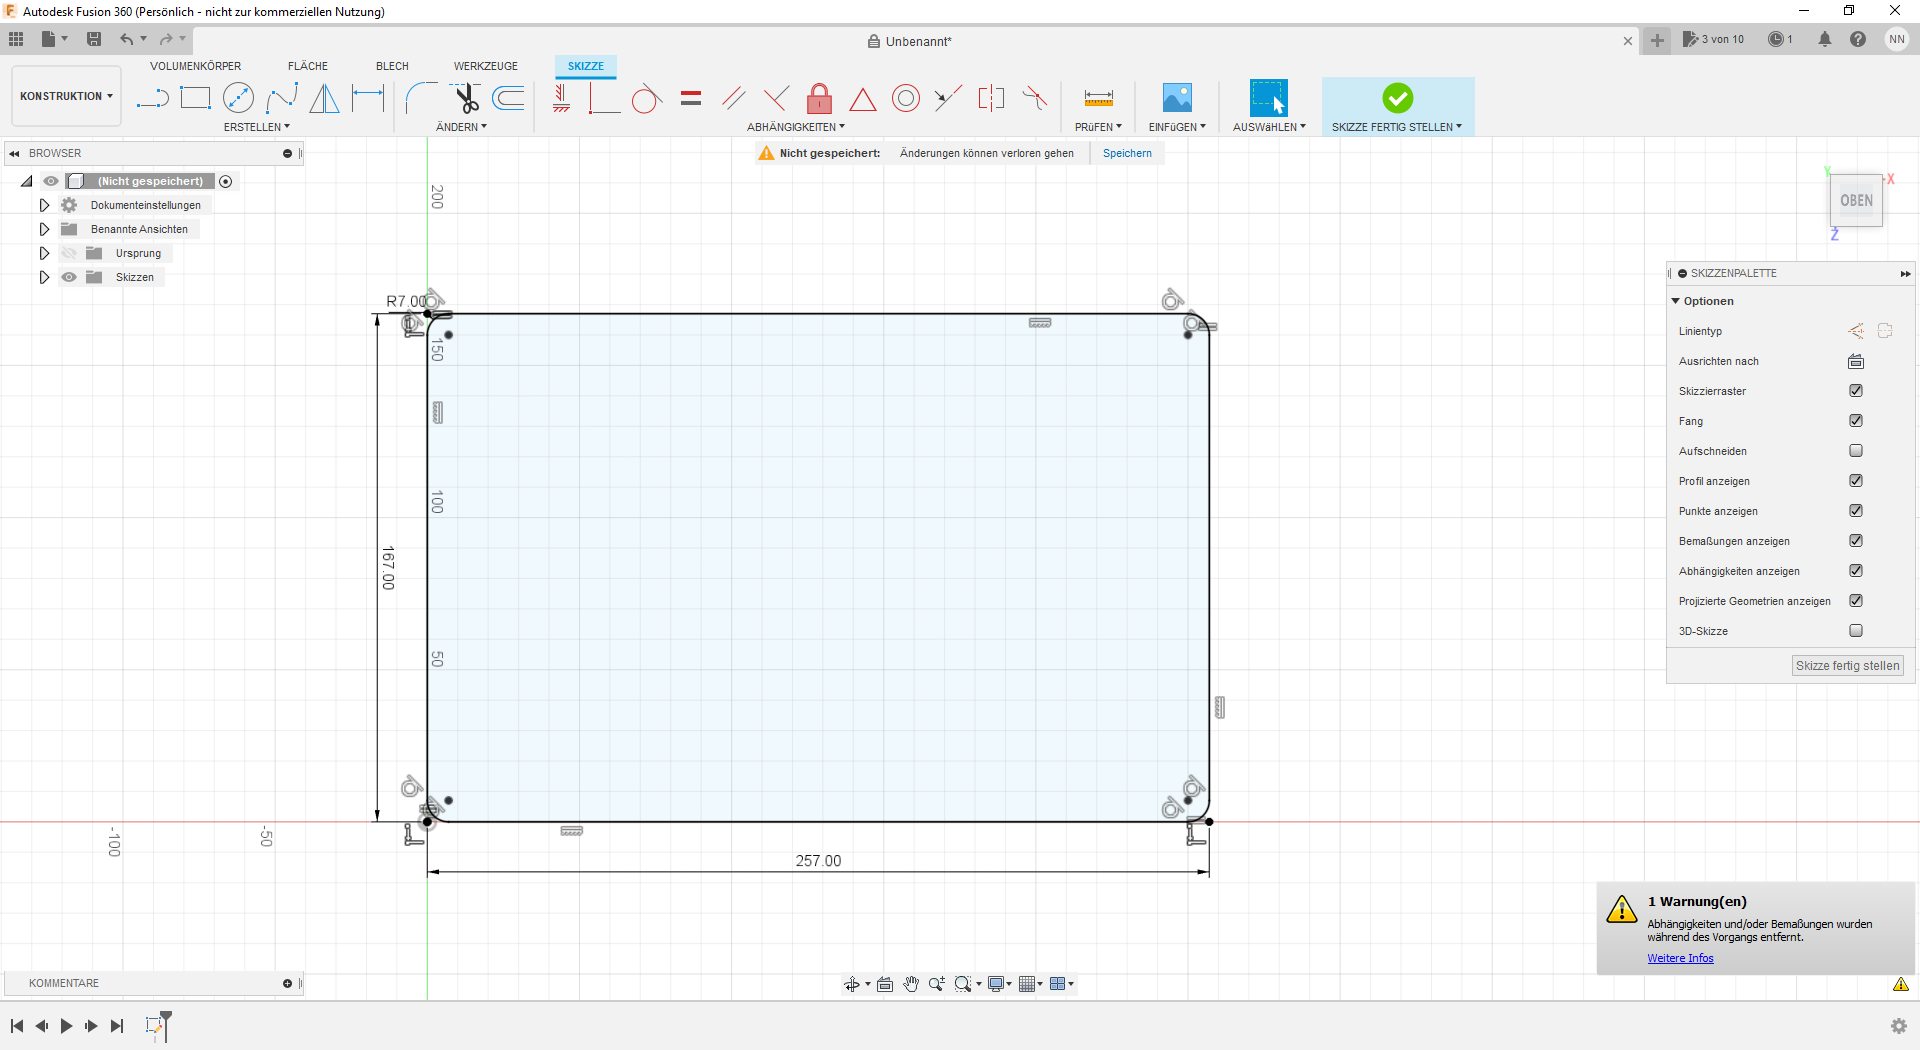
\includegraphics[width=1\textwidth]{img/konstruktion_gehaeuse_002.png}
		\caption[Abrunden der Ecken]{Abrunden der Ecken}
		\label{fig:design-case-02}
	\end{subfigure}
	\begin{subfigure}[b]{.5\linewidth}
		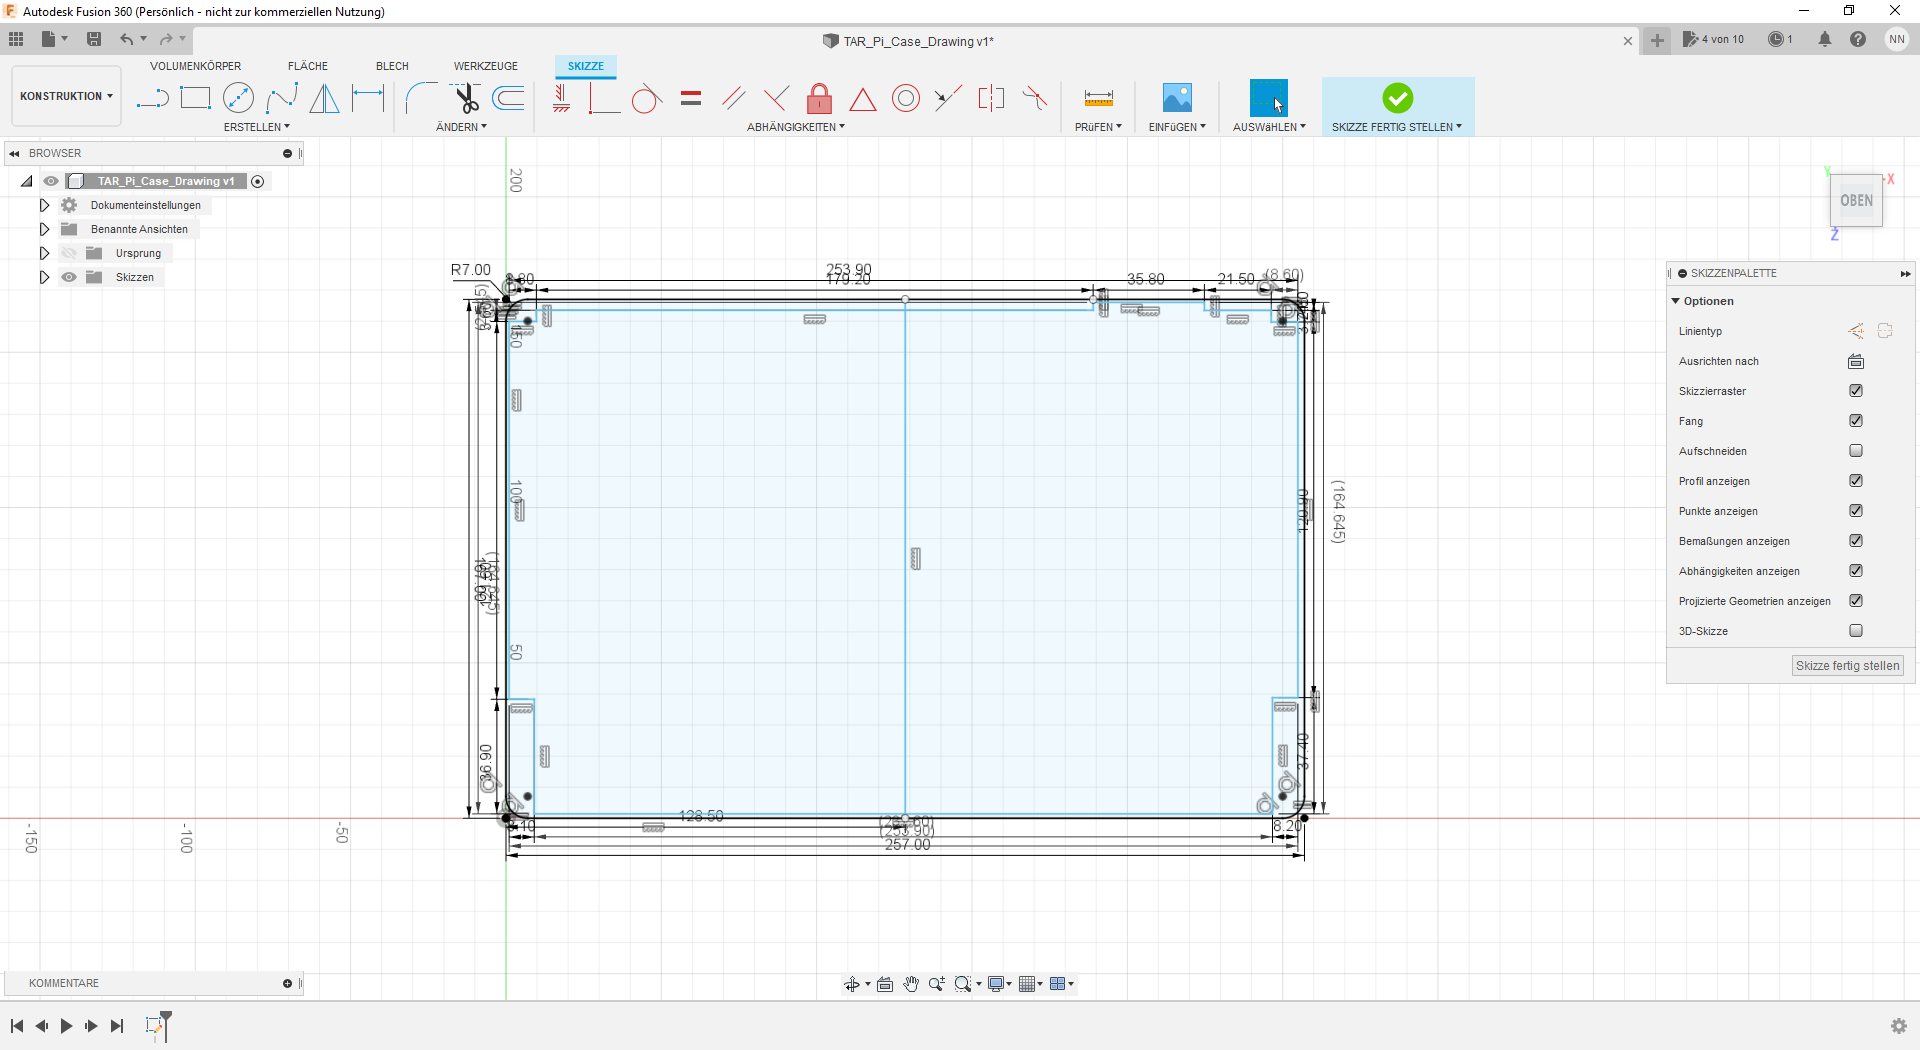
\includegraphics[width=1\textwidth]{img/konstruktion_gehaeuse_003.png}
		\caption[Zeichnen der Auflageflächen für das Gehäuse]{Zeichnen der Auflageflächen}
		\label{fig:design-case-03}
	\end{subfigure}
	\caption[Grundzeichnung als Basis des Modells]{Grundzeichnung als Basis des Modells}
	\label{fig:design-case-base}
\end{figure}\par
Die so entstandene Zeichnung (vgl. \ref{fig:design-case-03}) wurde dann in eine weitere Datei kopiert um als Grundlage für die beiden geteilten Seitenteile zu dienen. Von hier aus wurden die beiden Wand-Teile mehr oder weniger unabhängig voneinander entworfen.\par
\paragraph{Linkes Wandteil}
Beim linken Wandteil wurde der entsprechende Teil der Zeichnung um 2 mm entlang der Z-Achse extrudiert (vgl. \ref{fig:design-left-01}). Auf der erhöhten Seite wurde darauf hin eine weitere Zeichnung gelegt, die die Bleche an der Rückseite des Bildschirms überdecken sollte (vgl. \ref{fig:design-left-02}), die dann wie zuvor um 3 mm entlang der Z-Achse extrudiert wurde (vgl. \ref{fig:design-left-03}). Diese sollte dem Gehäuse genug Auflagefläche an dem Bildschirm bieten, um die Verklebung so stark wie möglich zu machen. Auf die nun entstandene erhöhte Seite wurde eine Zeichnung der ,,tatsächlichen'' Wandstärke von 3 mm erstellt (vgl. \ref{fig:design-left-04}). Diese wurde dann um 6 mm entlang der Z-Achse extrudiert, um für die Verbinder genügend Platz vor dem klobigen Blechbereich im unteren Teil des Bildschirms zu bieten (vgl. \ref{fig:design-left-05}). Auf die nun obenliegende Seite wurde die Zeichnung der Verbindungsstücke gelegt (vgl. \ref{fig:design-left-06}) und um 19 mm entlang der Z-Achse extrudiert (vgl. \ref{fig:design-left-07}) und im Kreismittelpunkt der Zeichnungen eine Bohrung für M3-Gewinde gesetzt (vgl. \ref{fig:design-left-08}). Auf die nun  entstandene Oberfläche wurde die Zeichnung für die Deckelverbindung gesetzt (vgl. \ref{fig:design-left-09}), um 25 mm entlang der Z-Achse extrudiert (vgl. \ref{fig:design-left-10}) und ebenfalls mit Bohrungen für M3-Gewinde versehen (vgl. \ref{fig:design-left-11}).
%beschreibungstext links
\begin{figure}[h!tb]
	\begin{subfigure}[t]{.3\linewidth}
		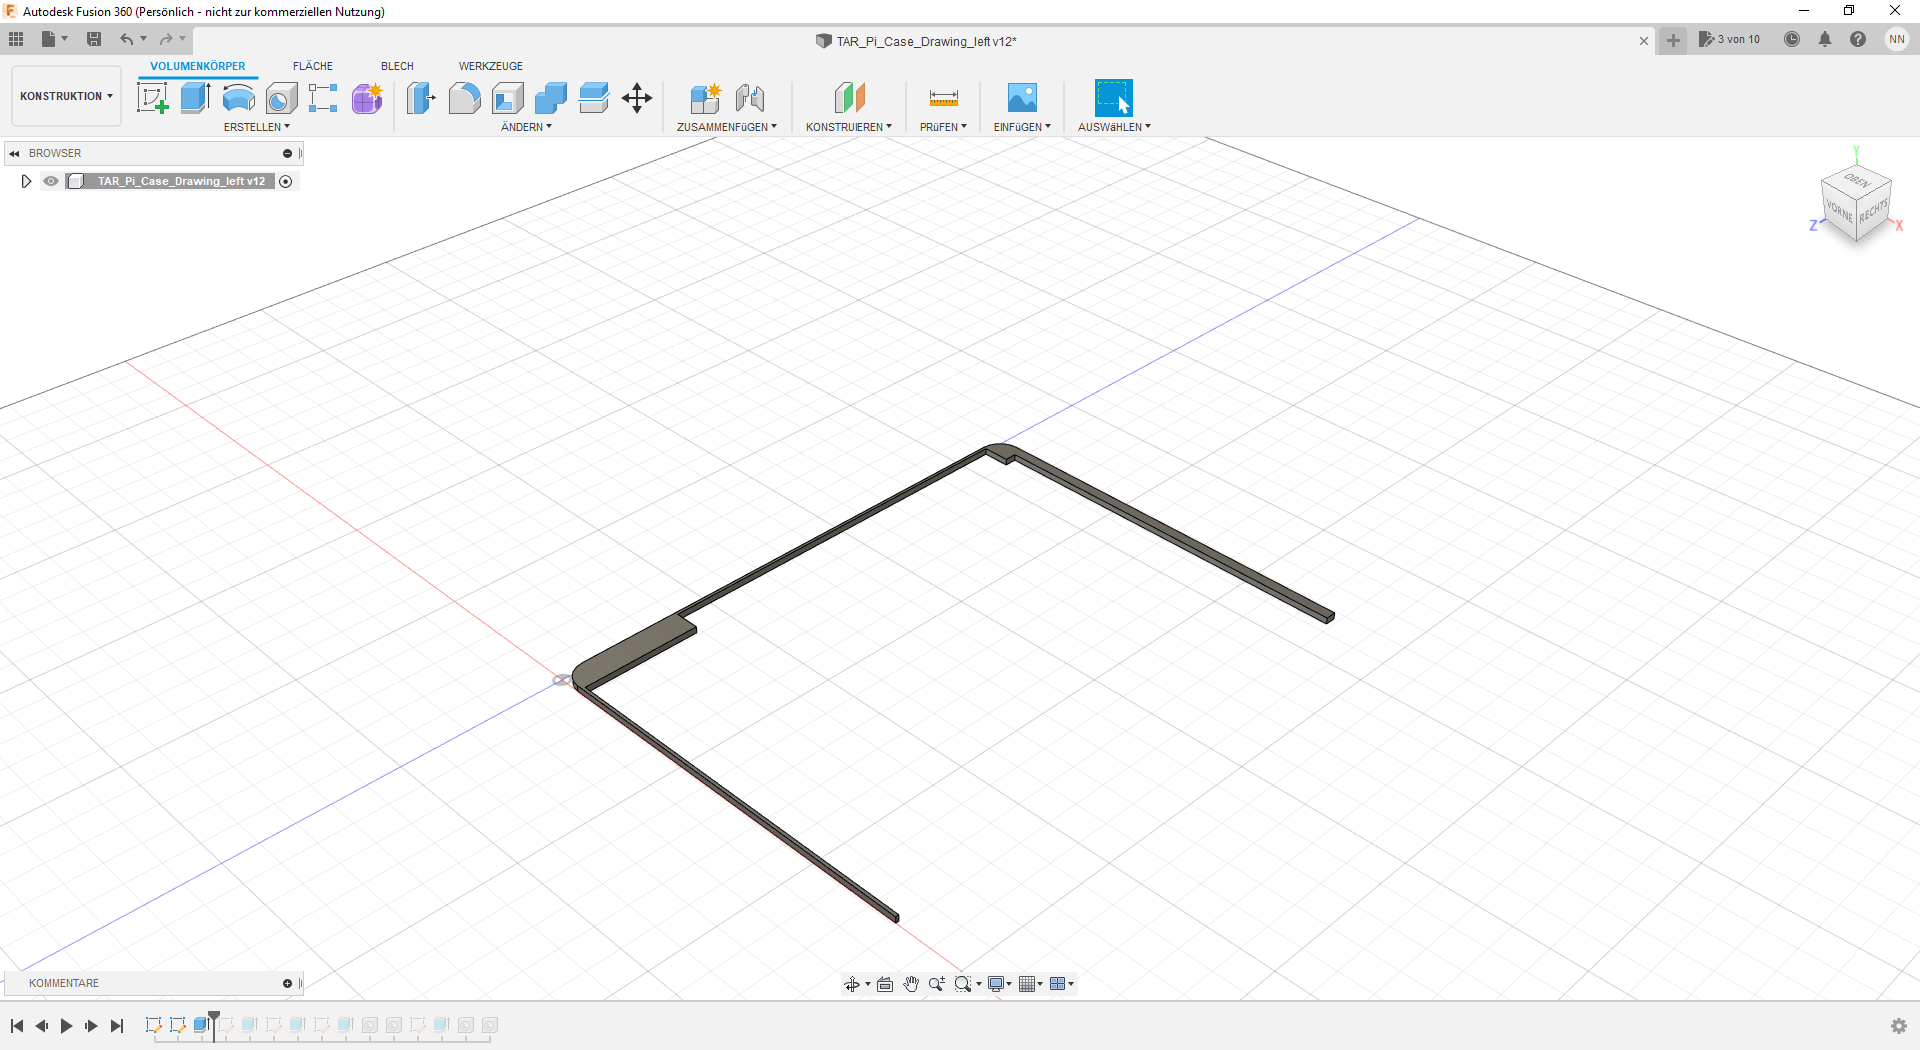
\includegraphics[width=\linewidth]{img/konstruktion_gehaeuse_links_001.png}
		\caption[Extrusion der Grundzeichnung]{Extrusion der Grundzeichnung}
		\label{fig:design-left-01}
	\end{subfigure}
	\begin{subfigure}[t]{.3\linewidth}
		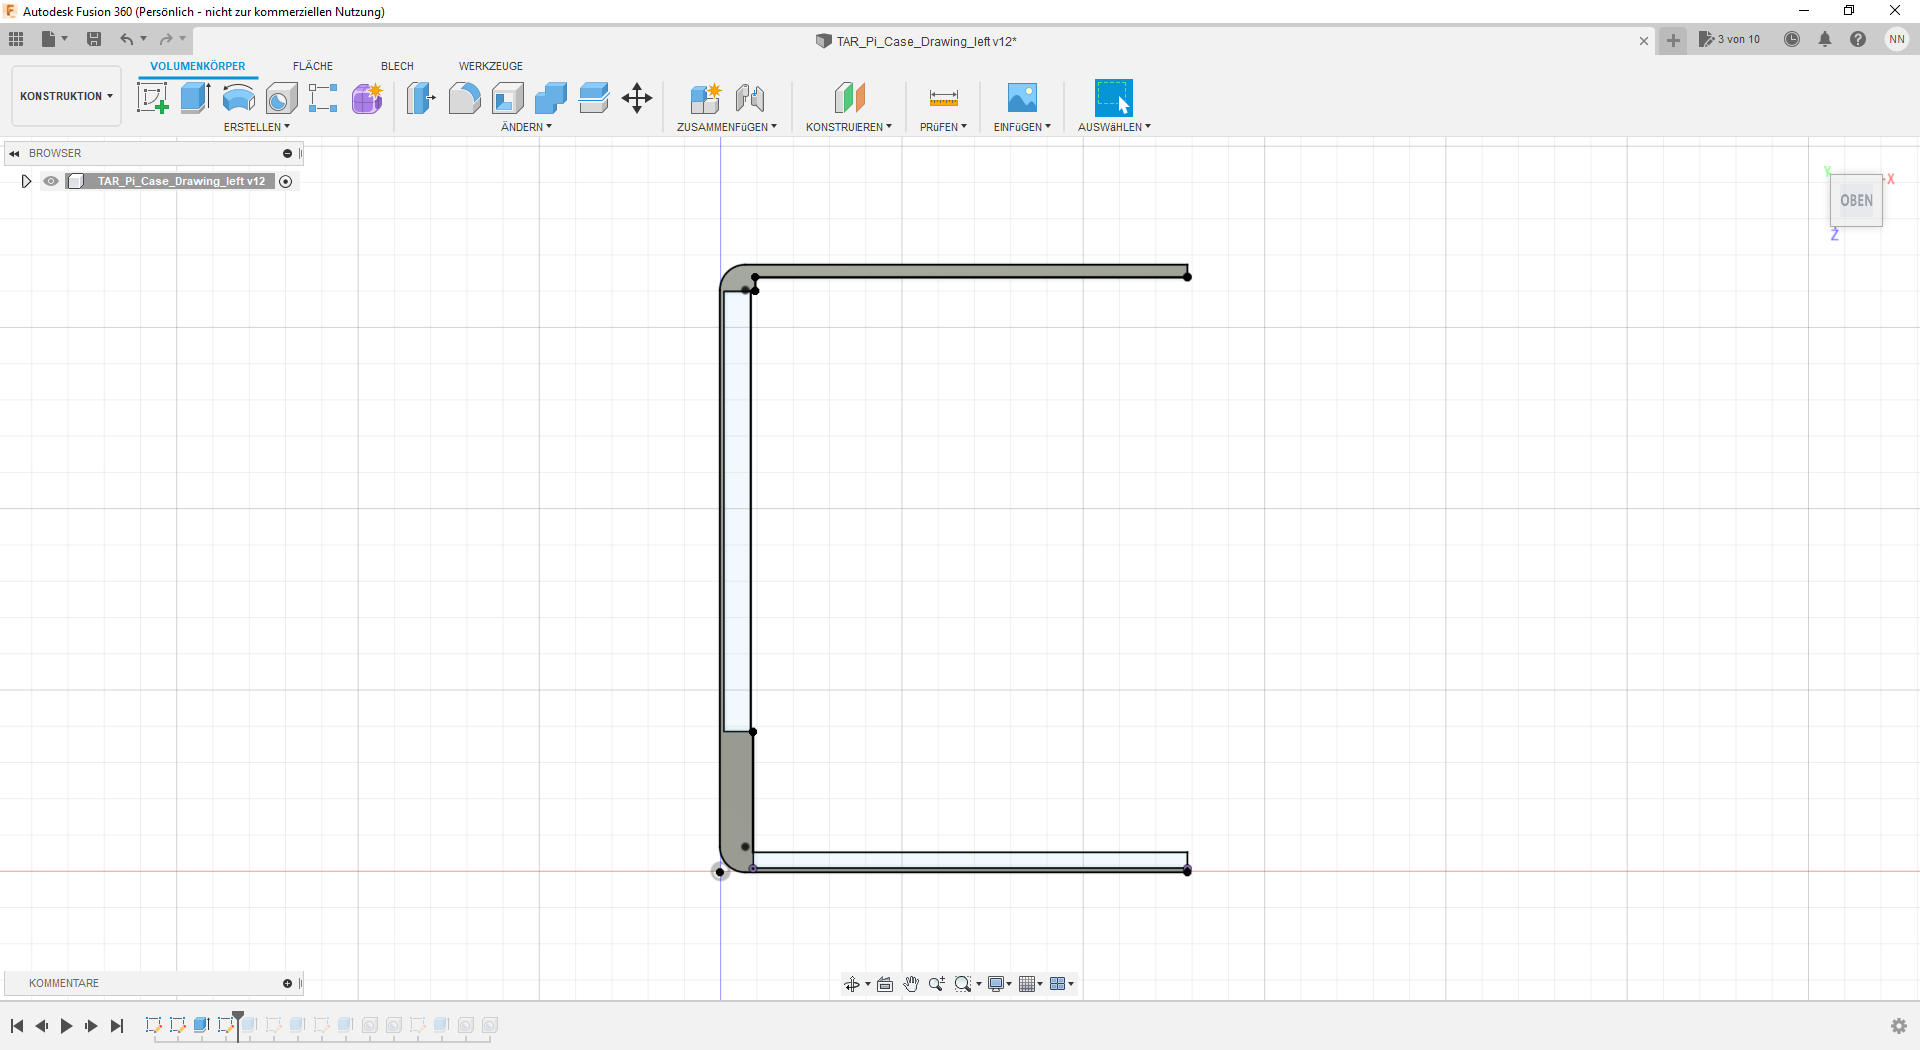
\includegraphics[width=\linewidth]{img/konstruktion_gehaeuse_links_002.png}
		\caption[Erstellung der Folgezeichnung um Blech]{Erstellung der Folgezeichnung um Blech}
		\label{fig:design-left-02}
	\end{subfigure}
	\begin{subfigure}[t]{.3\linewidth}
		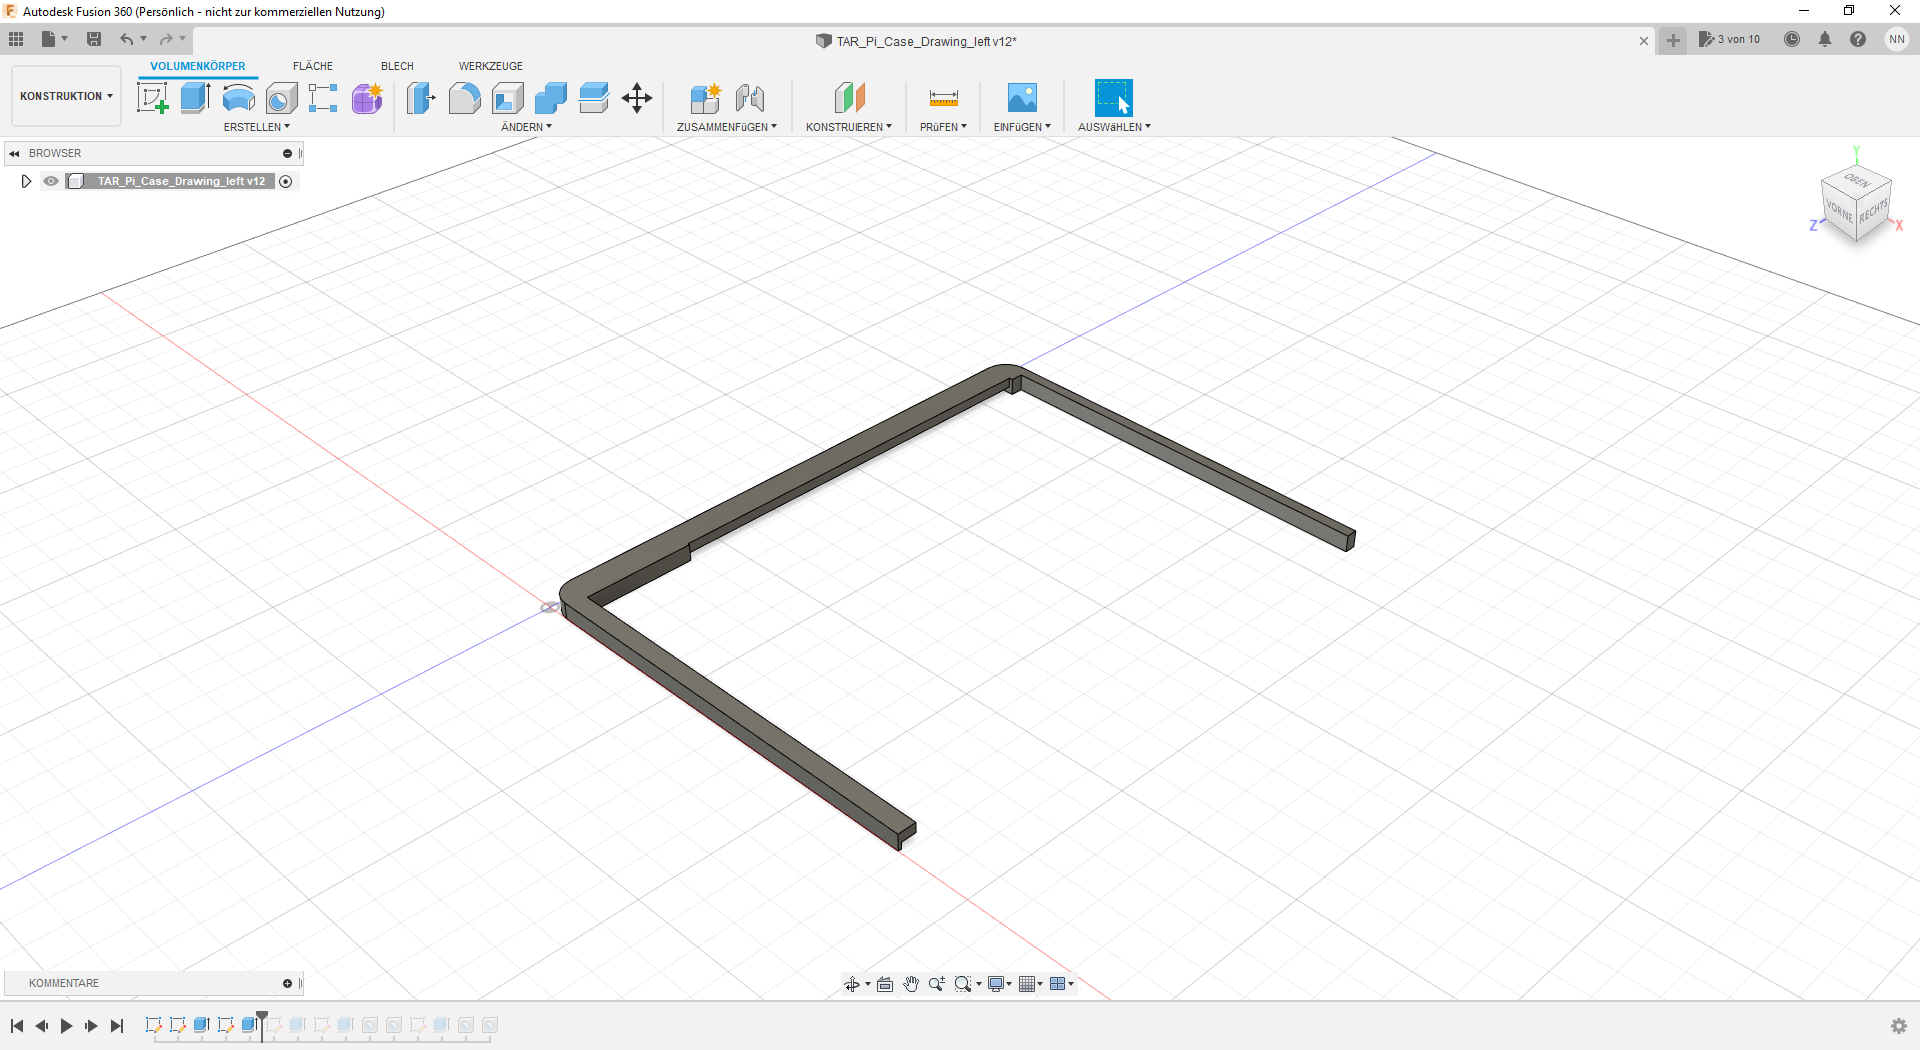
\includegraphics[width=\linewidth]{img/konstruktion_gehaeuse_links_003.png}
		\caption[Extrusion der neuen Zeichnung]{Extrusion der neuen Zeichnung}
		\label{fig:design-left-03}
	\end{subfigure}
	\begin{subfigure}[t]{.3\linewidth}
		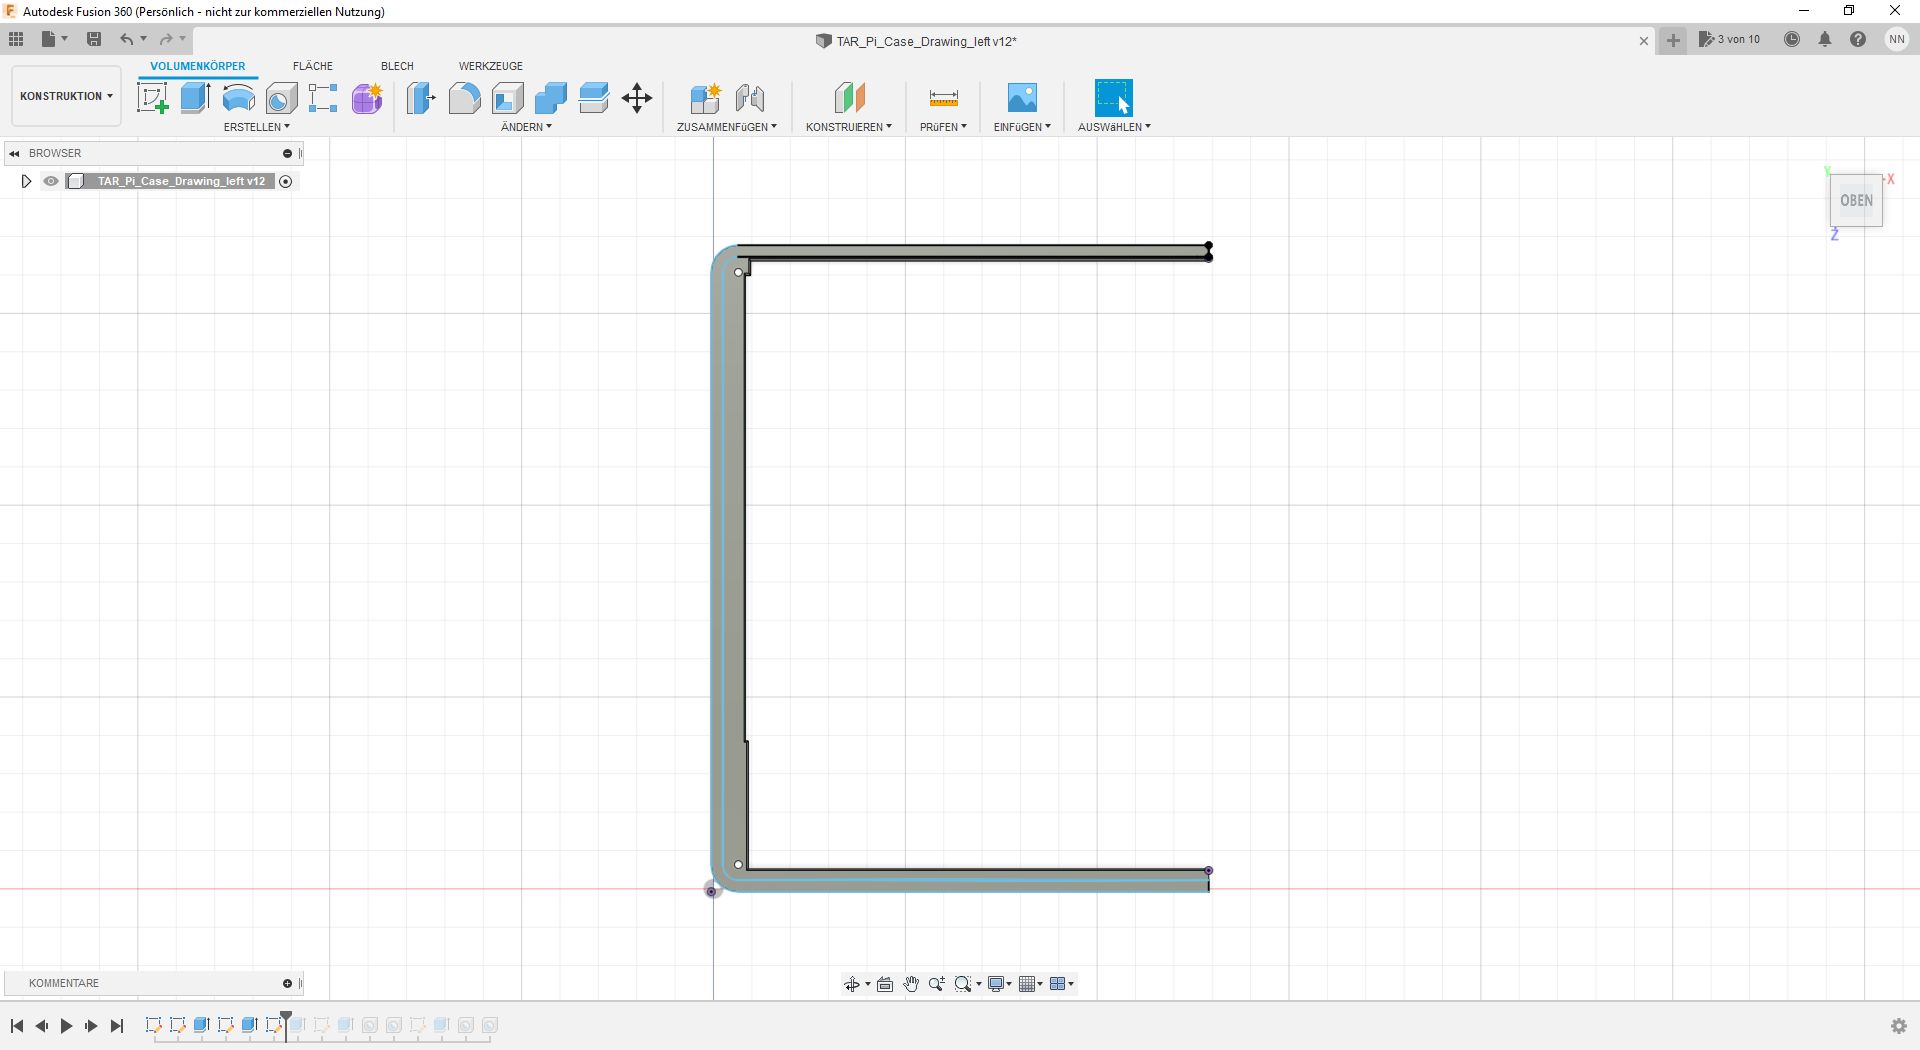
\includegraphics[width=\linewidth]{img/konstruktion_gehaeuse_links_004.png}
		\caption[Zeichnung der Hauptwandstärke]{Zeichnung der Hauptwandstärke}
		\label{fig:design-left-04}
	\end{subfigure}
	\begin{subfigure}[t]{.3\linewidth}
		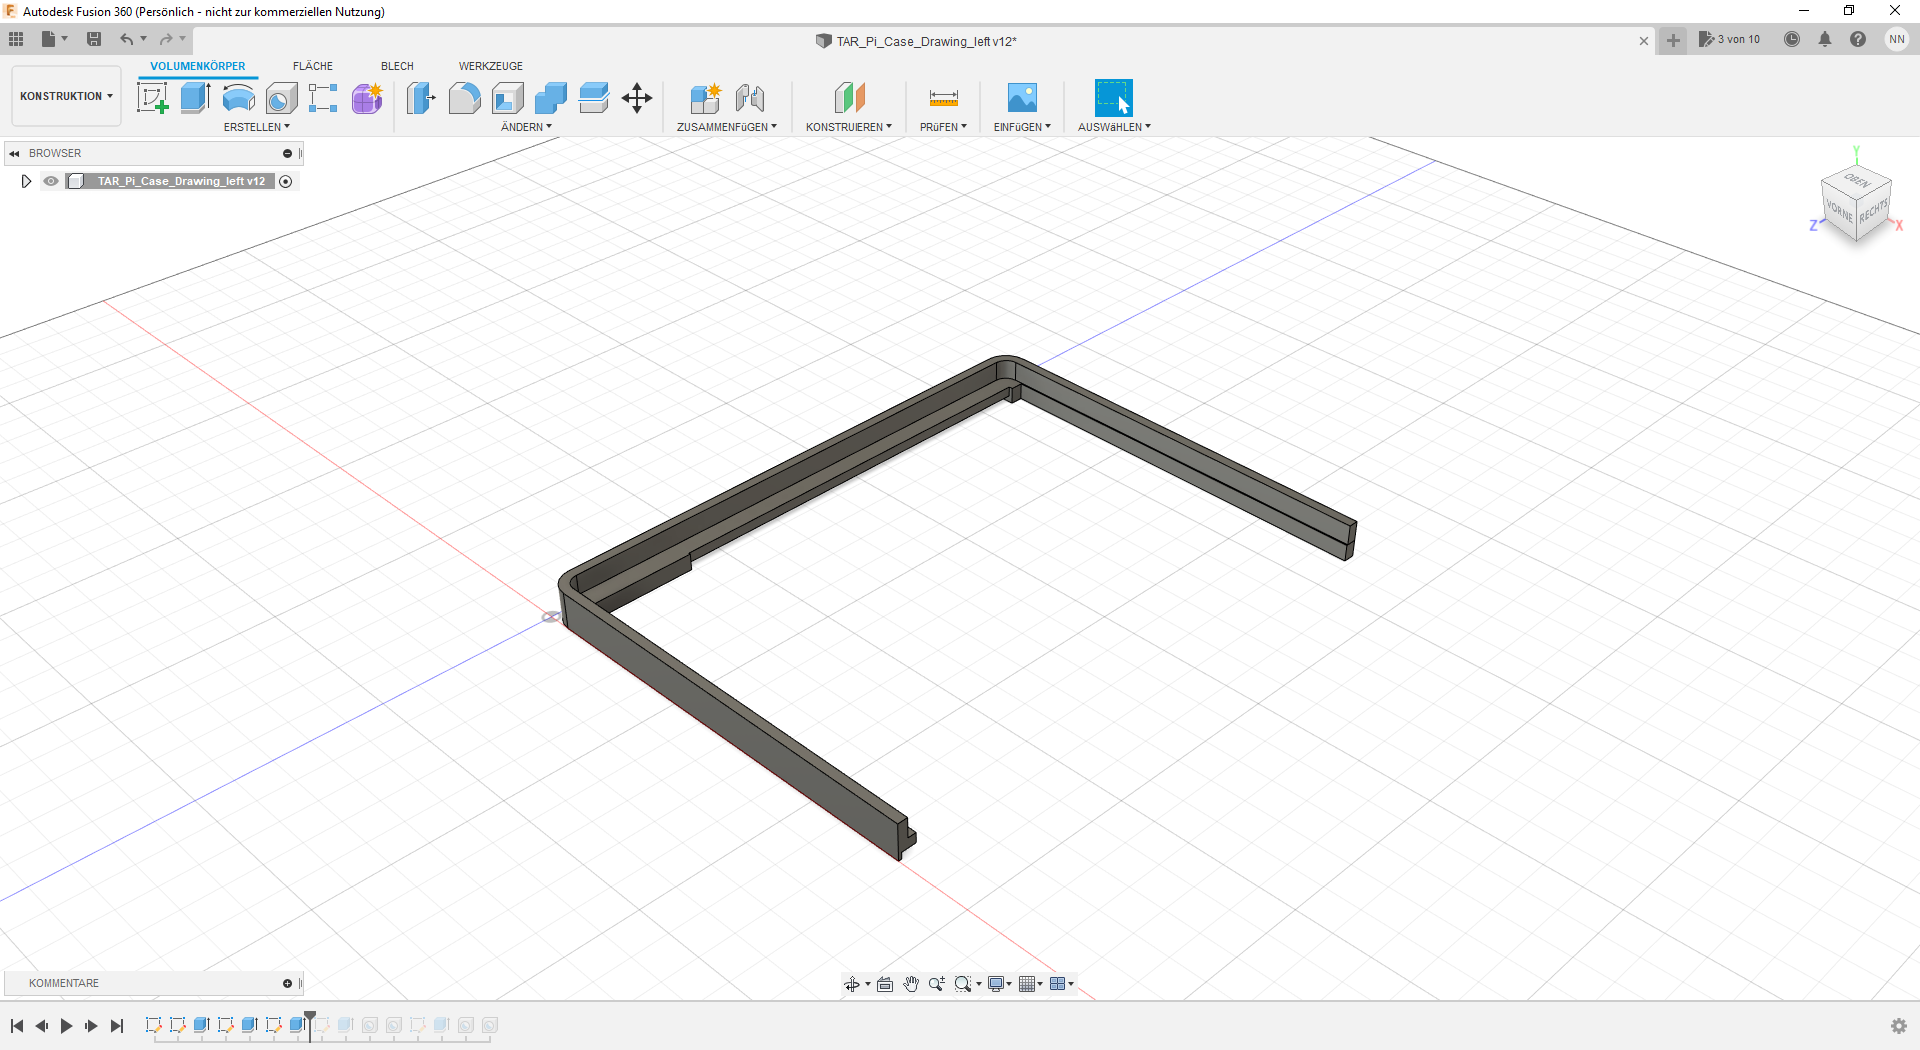
\includegraphics[width=\linewidth]{img/konstruktion_gehaeuse_links_005.png}
		\caption[Extrusion der Hauptwand]{Extrusion der Hauptwand}
		\label{fig:design-left-05}
	\end{subfigure}
	\begin{subfigure}[t]{.3\linewidth}
		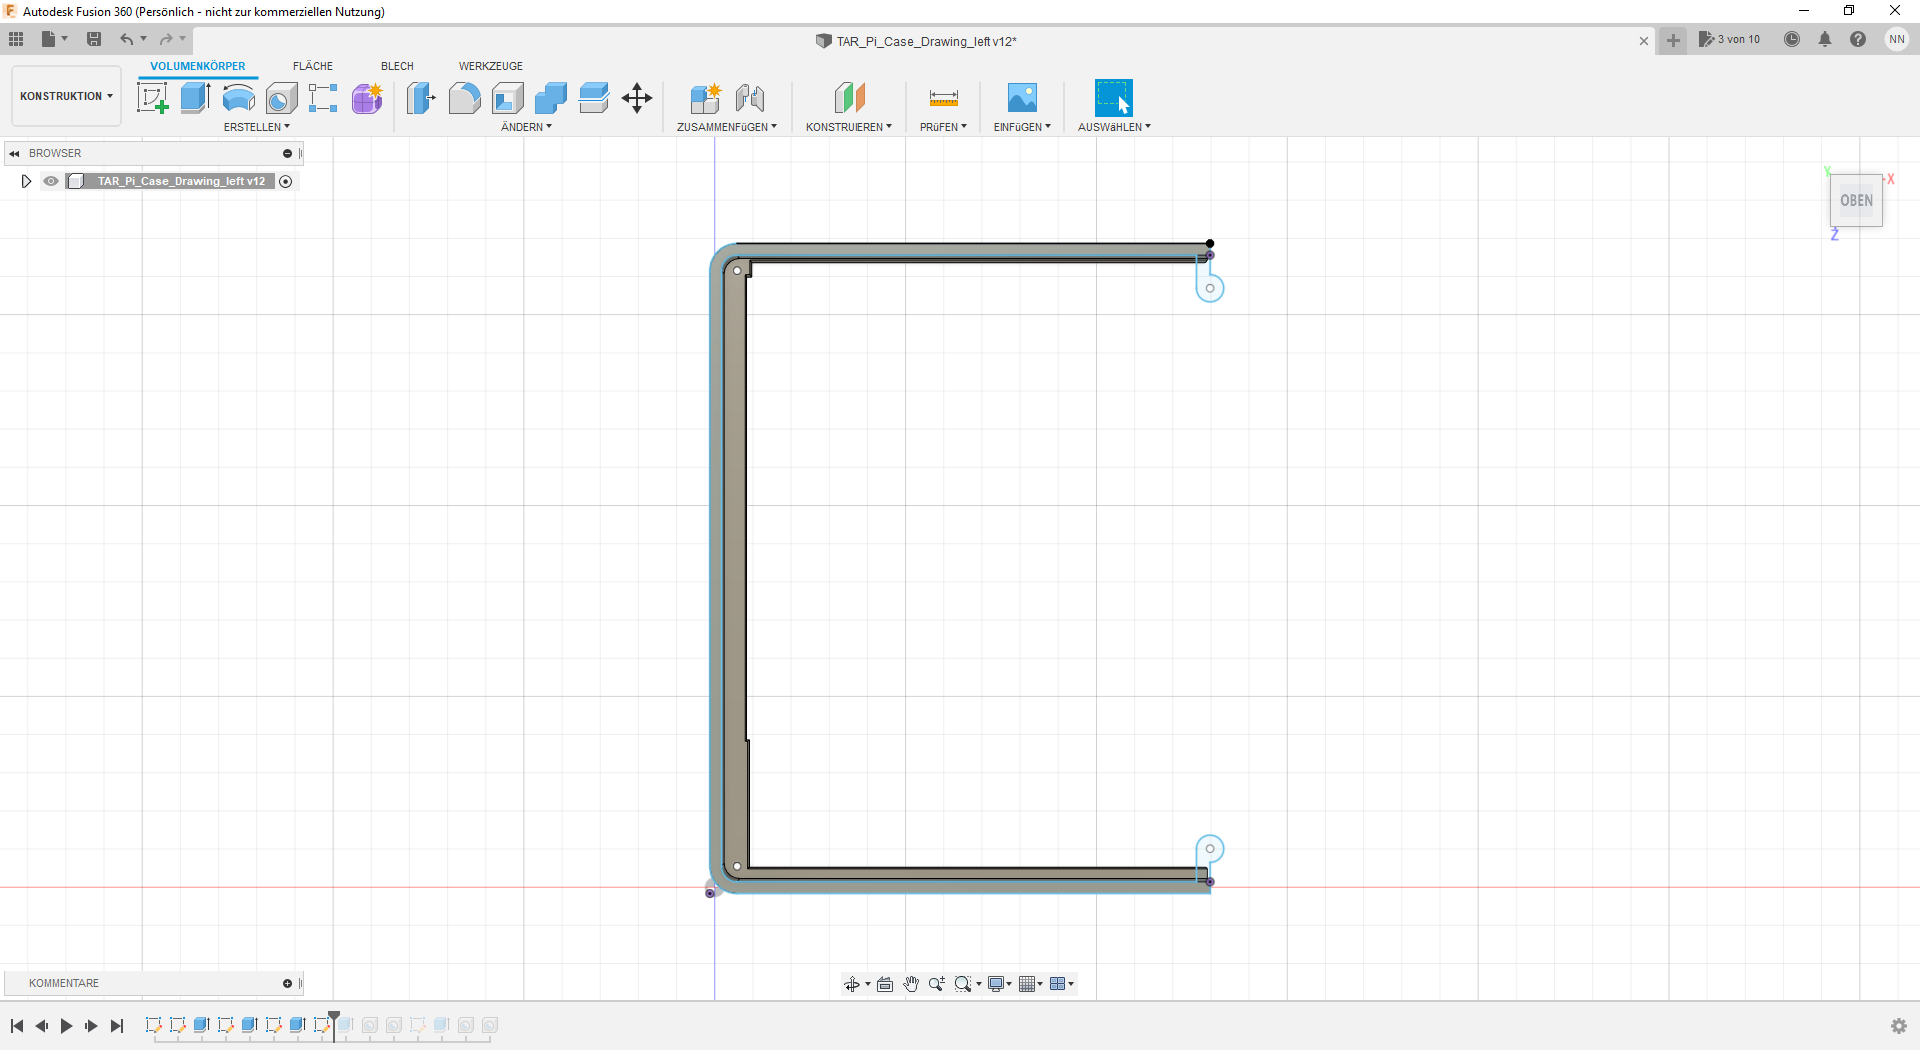
\includegraphics[width=\linewidth]{img/konstruktion_gehaeuse_links_006.png}
		\caption[Zeichnung der Verbindungsstücke]{Zeichnung der Verbindungsstücke}
		\label{fig:design-left-06}
	\end{subfigure}
	\begin{subfigure}[t]{.3\linewidth}
		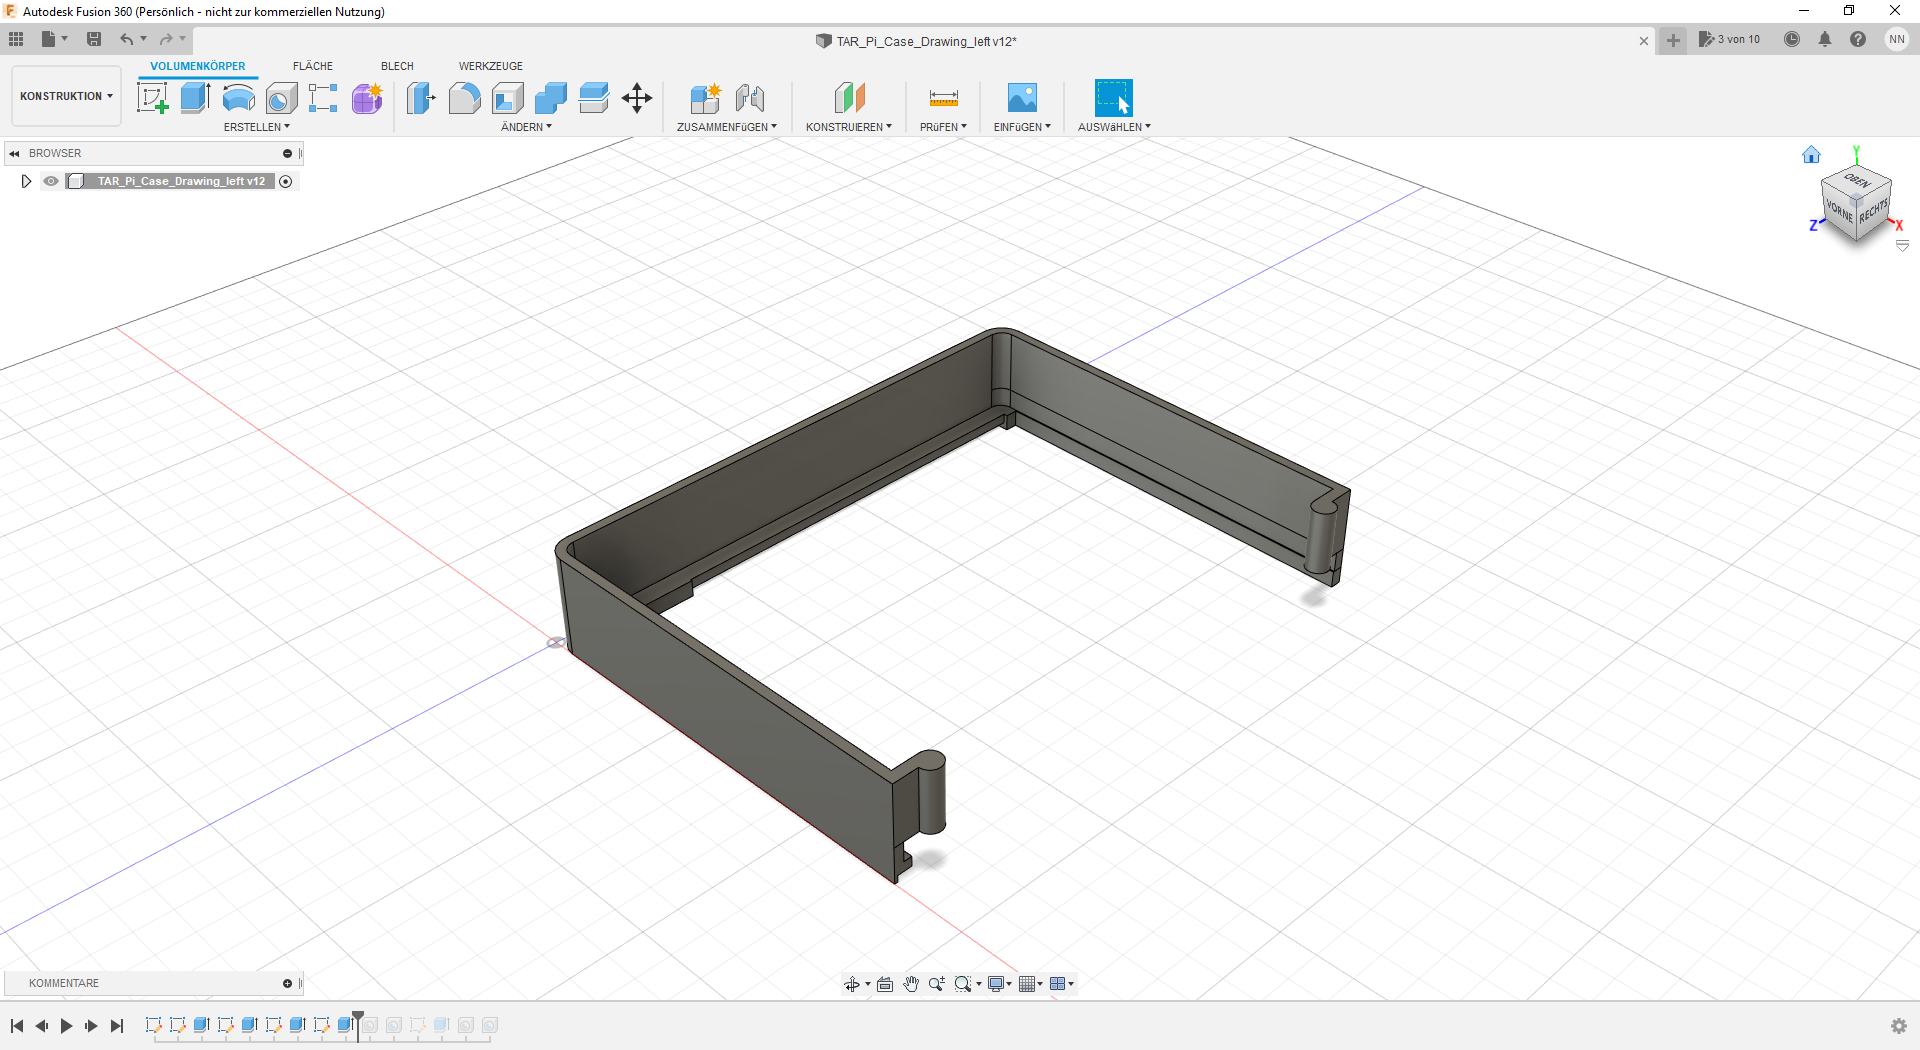
\includegraphics[width=\linewidth]{img/konstruktion_gehaeuse_links_007.png}
		\caption[Extrusion der Hauptwand mit Verbindungsstücken]{Extrusion der Hauptwand mit Verbindungsstücken}
		\label{fig:design-left-07}
	\end{subfigure}
	\begin{subfigure}[t]{.3\linewidth}
		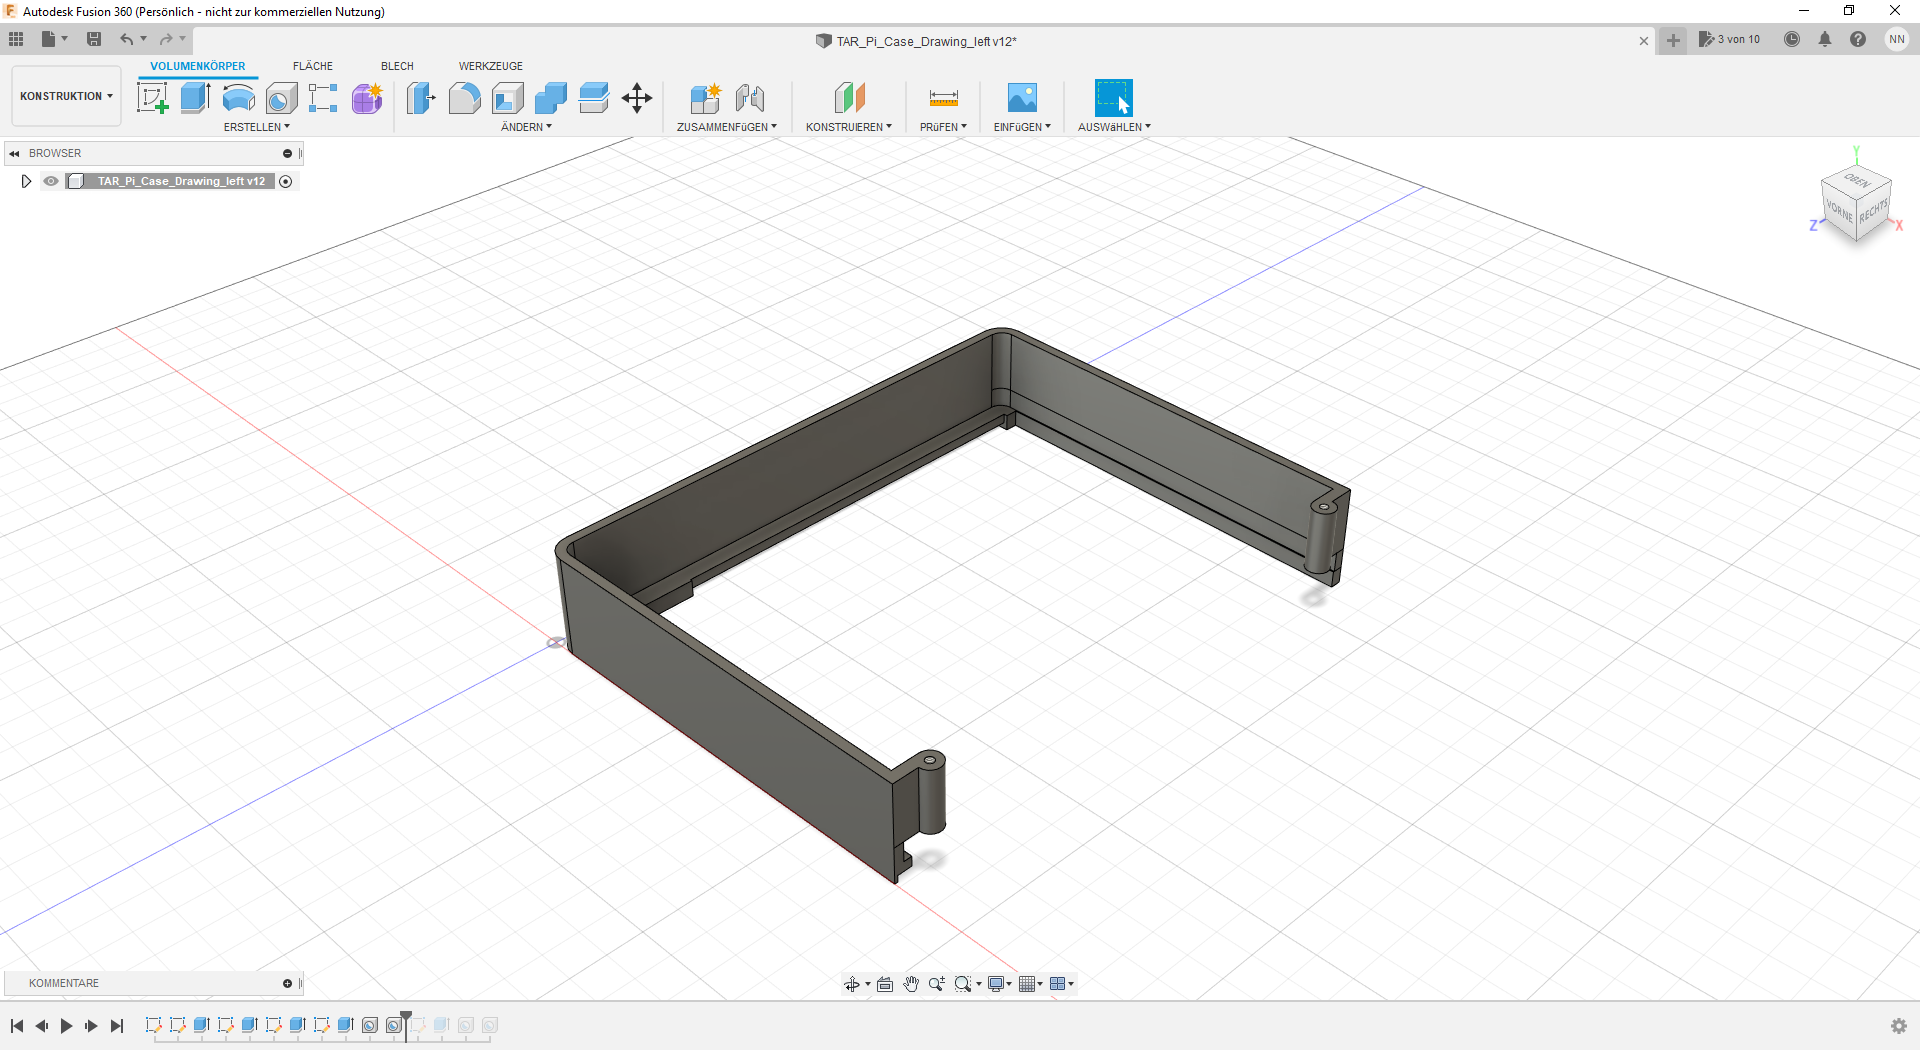
\includegraphics[width=\linewidth]{img/konstruktion_gehaeuse_links_008.png}
		\caption[Bohrung für Schrauben]{Bohrung für Schrauben}
		\label{fig:design-left-08}
	\end{subfigure}
	\begin{subfigure}[t]{.3\linewidth}
		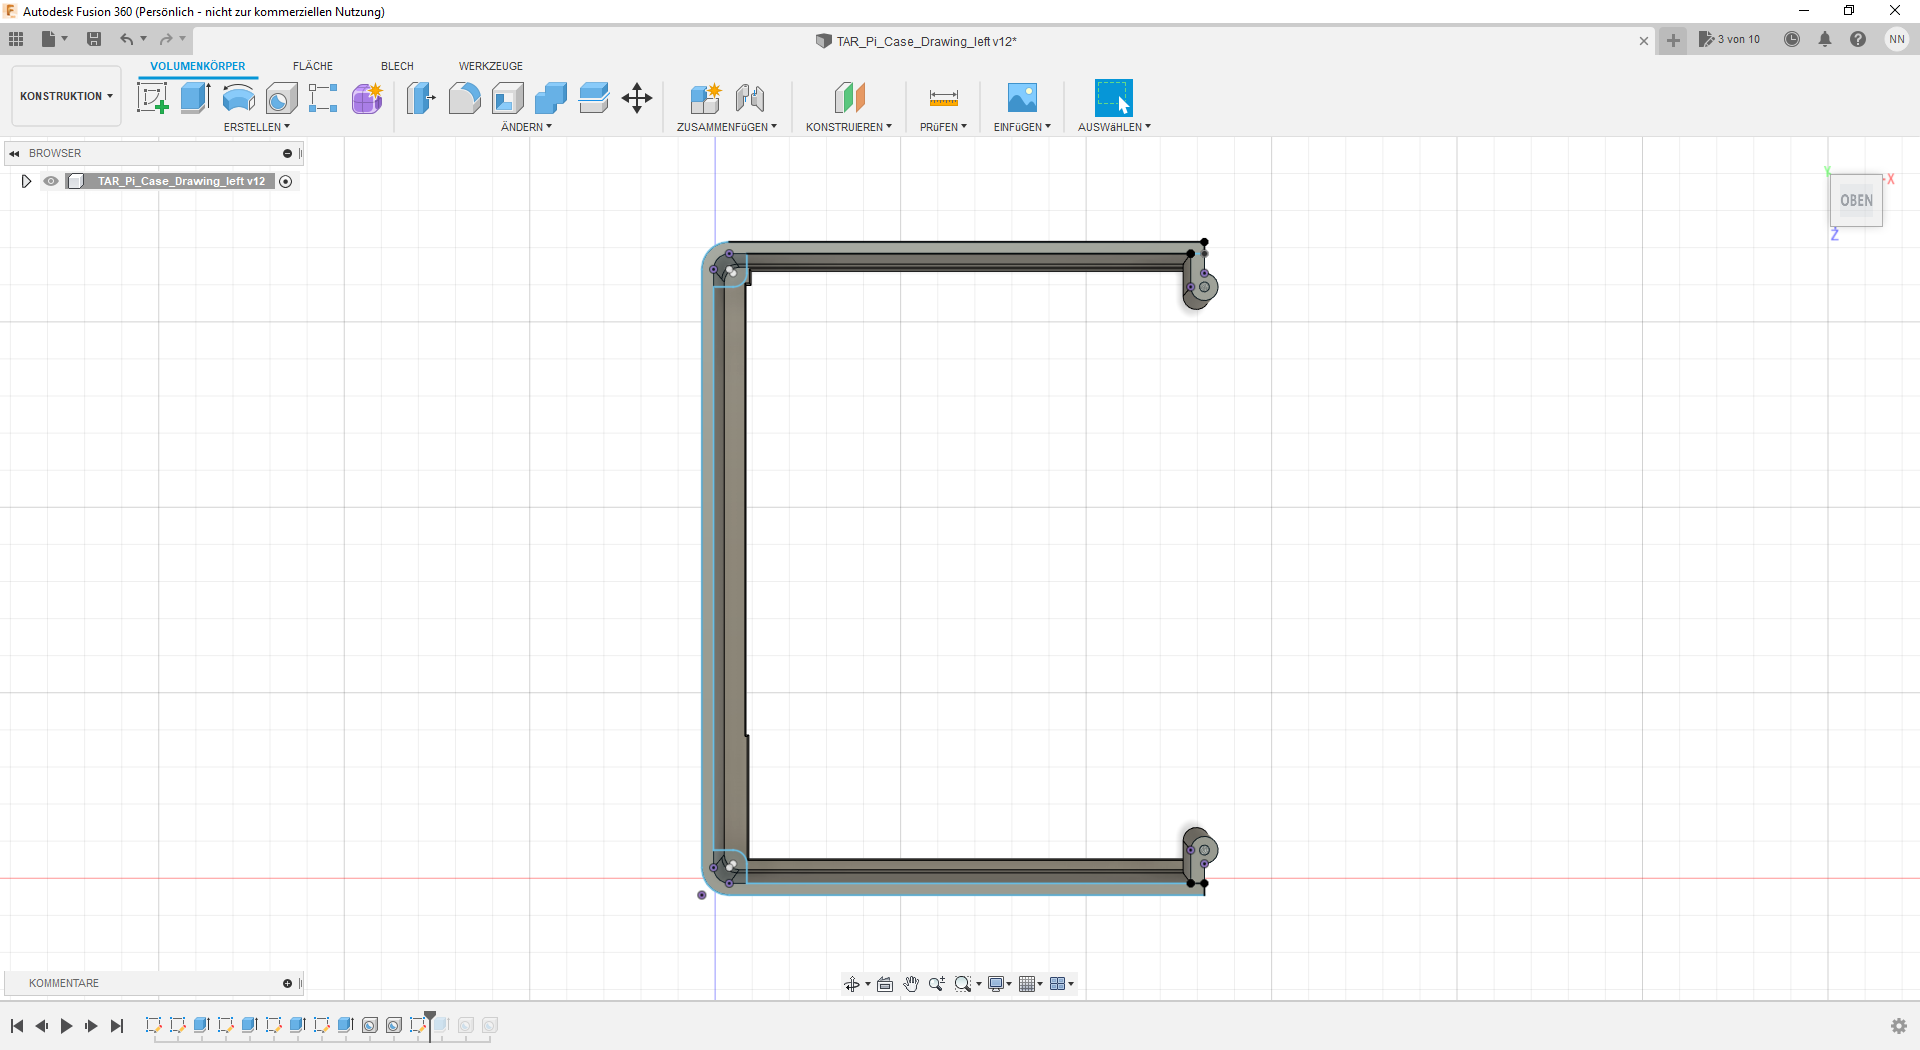
\includegraphics[width=\linewidth]{img/konstruktion_gehaeuse_links_009.png}
		\caption[Zeichnung der Deckelverbindung]{Zeichnung der Deckelverbindung}
		\label{fig:design-left-09}
	\end{subfigure}
	\begin{subfigure}[t]{.3\linewidth}
		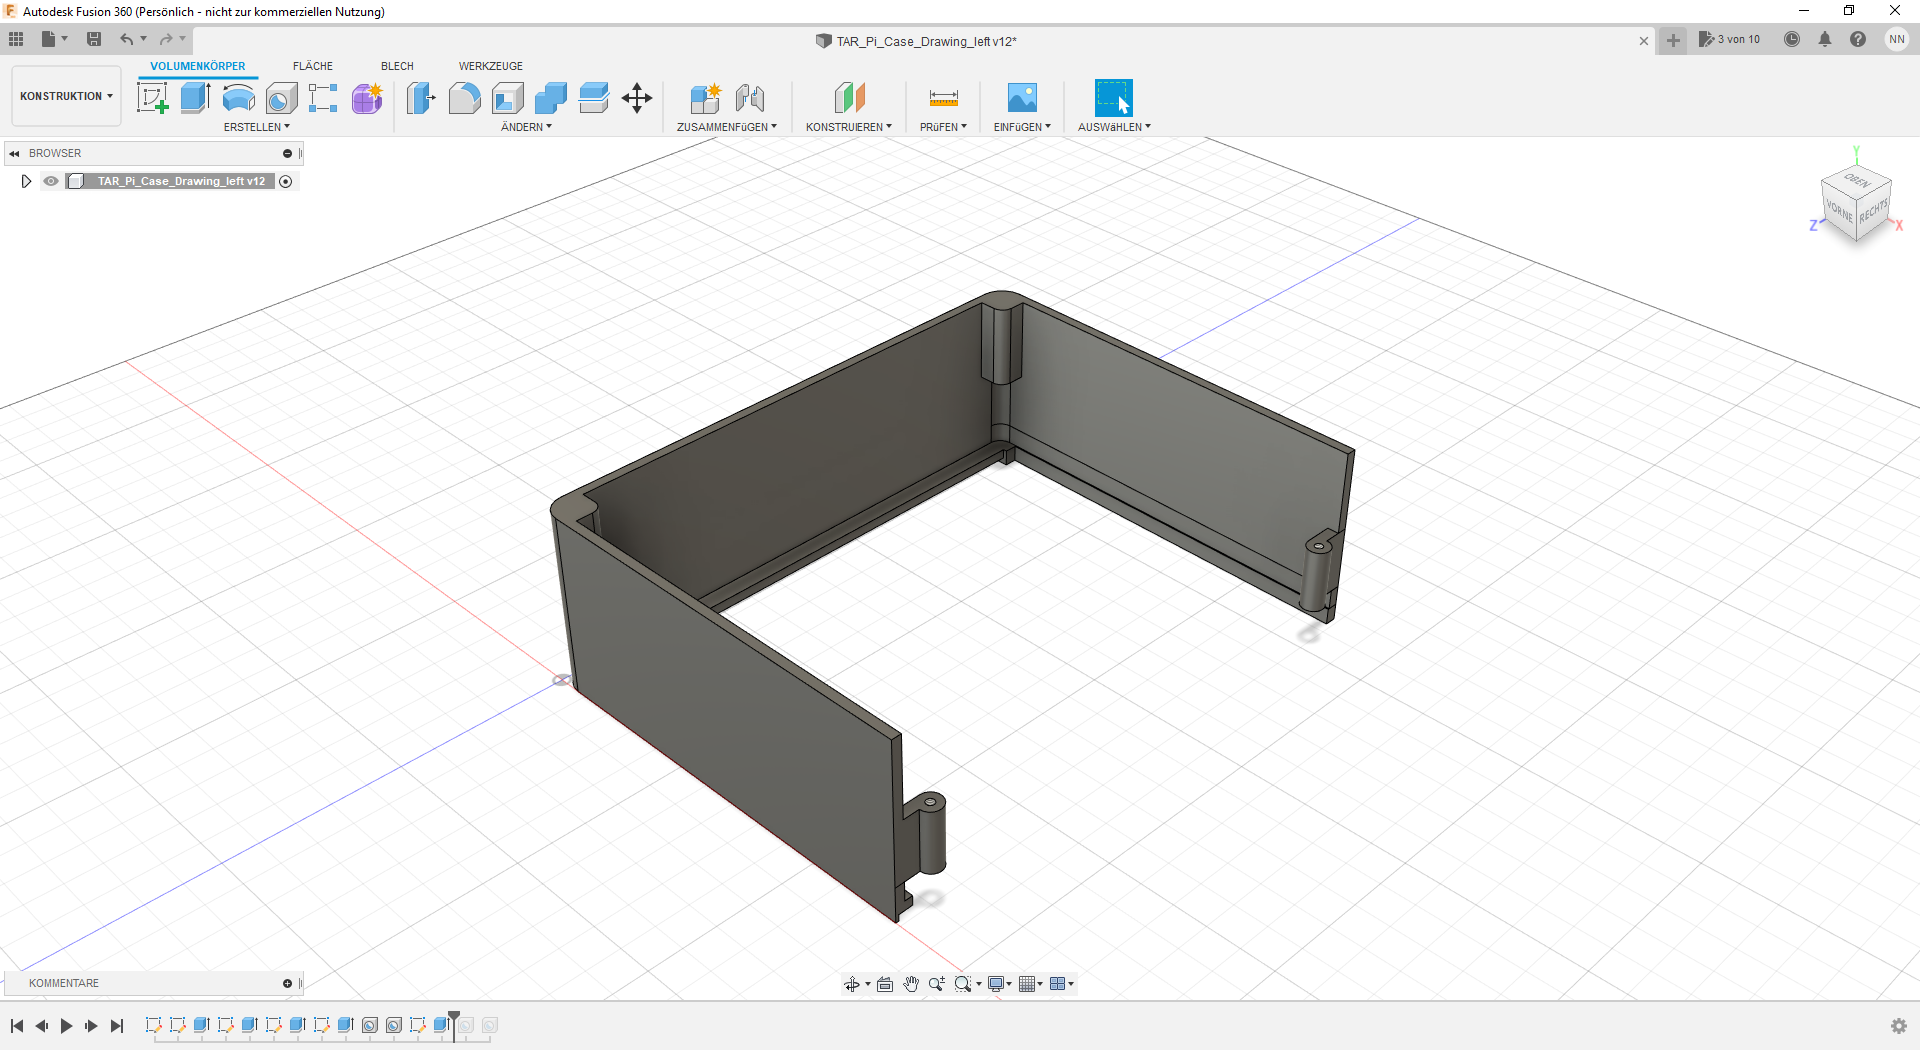
\includegraphics[width=\linewidth]{img/konstruktion_gehaeuse_links_010.png}
		\caption[Extrusion der Hauptwand mit Deckelverbindung]{Extrusion der Hauptwand mit Deckelverbindung}
		\label{fig:design-left-10}
	\end{subfigure}
	\begin{subfigure}[t]{.3\linewidth}
		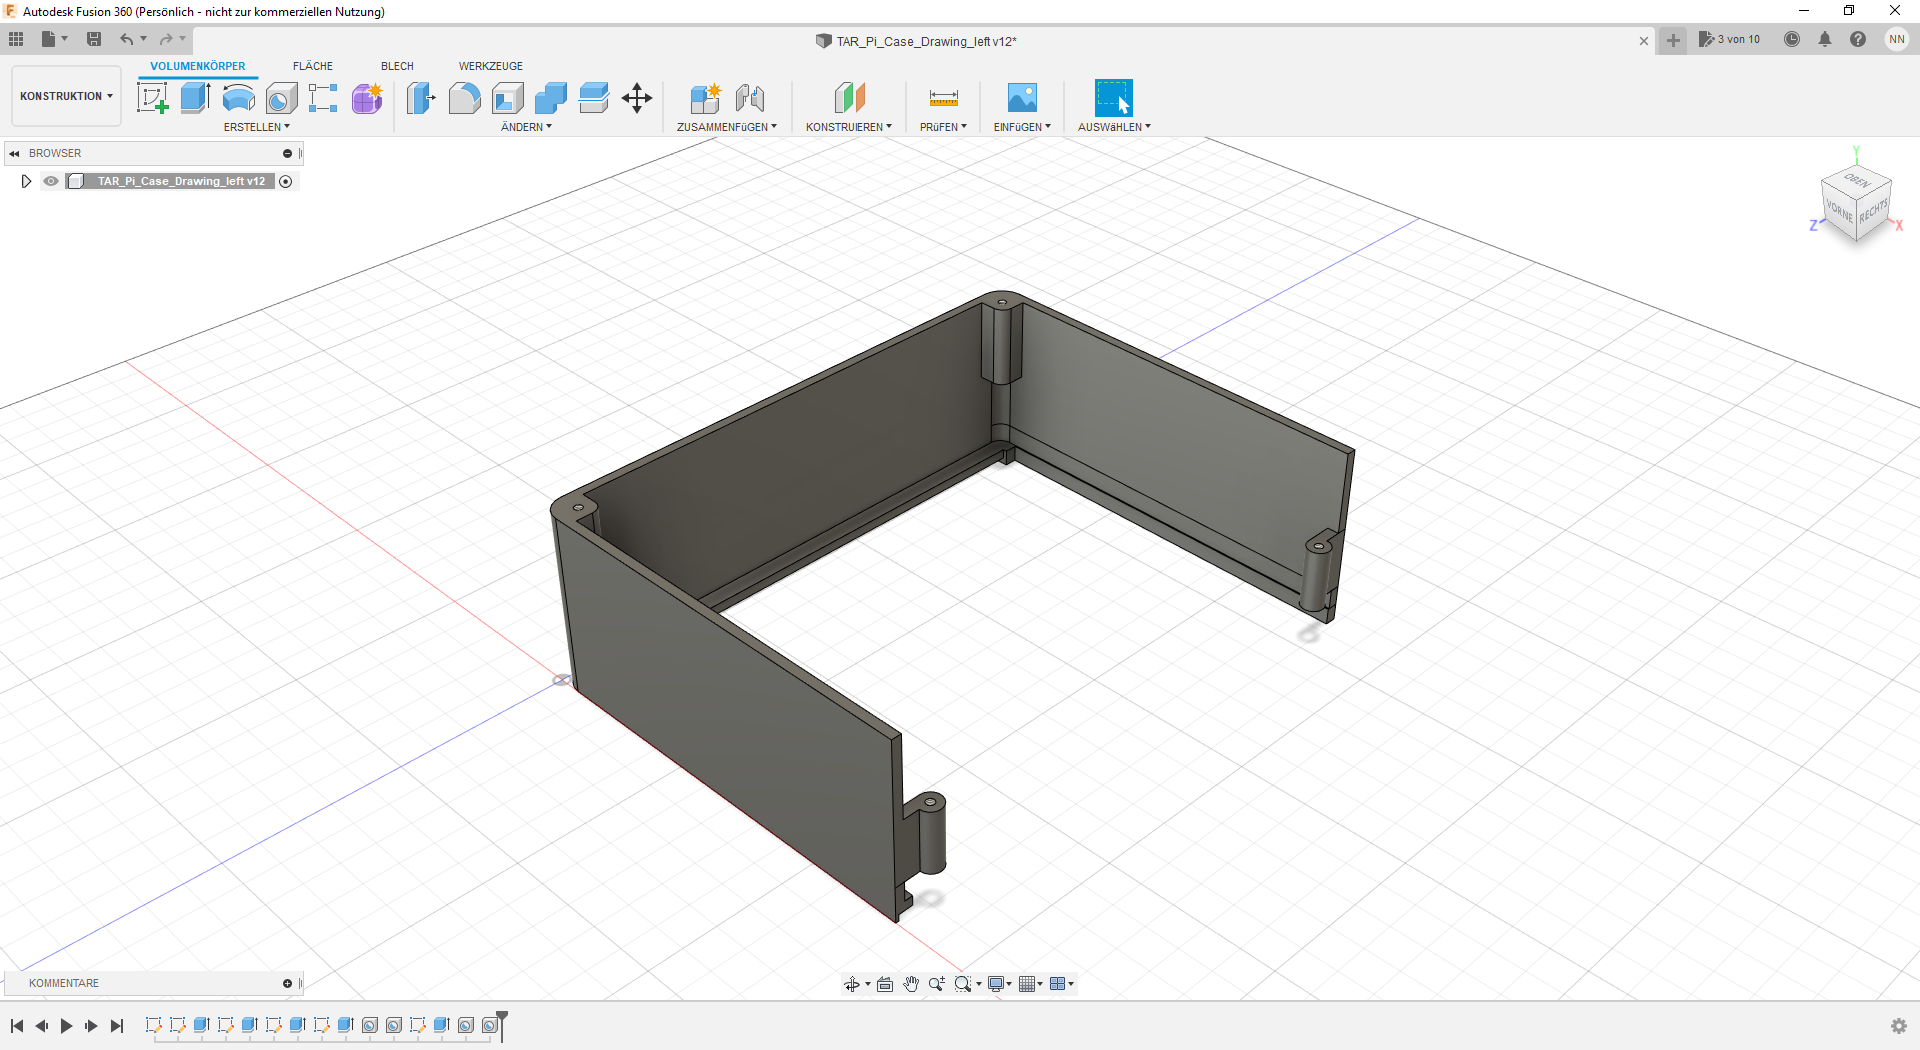
\includegraphics[width=\linewidth]{img/konstruktion_gehaeuse_links_011.png}
		\caption[Bohrungen der Deckelverbindung]{Bohrungen der Deckelverbindung}
		\label{fig:design-left-11}
	\end{subfigure}
	\caption[Entwurf des linken Wandteils]{Entwurf des linken Wandteils}
	\label{fig:design-left}
\end{figure}\par
\paragraph{Rechtes Wandteil}

\newpage